\chapter{Simulated Quadrant Photodiode}
\label{chapter:simulated_QPD}

\section{Introduction}
As demonstrated in Chapter 3, the motion and behaviour of a dimer 
is significantly different compared to that of a traditional sphere.
While this is simple enough to demonstrate in a simulation, where the 
position and orientation can be computed using the finite differences
method, from an experimental perspective these details can go unnoticed.
In order to accurately capture the dynamics of a trapped sphere, a 
position detection system is typically used - the most common of which is 
a Quadrant Photo Diode (QPD). A QPD sends a signal measuring 
the voltage difference between 4 photo diode quadrants. For purely 
translational motion the diodes can be split into neighbouring pairs 
(i.e. left and right, top and bottom - see Fig~\ref{fig:QPD_diagram})
to estimate the total displacement made by the target particle. 
However the same method cannot be applied to stochastic rotational 
motion. 

The relationship between particle translations and light scattering 
was first demonstrated by Rohrbach, where they showed a linear change 
in the scattered light when the particle was displaced \cite{Rohrbach2002}. They further showed that the optical force exerted by the trapping 
beam could be determined from the change in scattered light \cite{Rohrbach2002}. Rohrbach's model would later be used to develop 
modern position detection systems, where by calibrating the scattering 
signal using one of the many calibration techniques one could achieve a highly accurate estimation of the translational motion in the $X$-$Y$ 
plane.The most common of which being the Power Spectral Density method, 
one of the greatest advantages of the PSD method is that periodic 
rotational motion is also captured in the power spectrum. As an 
example consider an elongated cylindrical particle that is wobbling
around the $Z$-axis at some periodic frequency 'f'. A power spectrum 
of that trajectory will show a peak at that frequency. If however the 
wobble is periodic but instead stochastic, then it is impossible to 
separate out the rotational motion from the translational motion. This
poses some challenges to experimental modelling of non-spherical 
particles, if we cannot glean any information on the orientation
of the trapped particle we cannot accurately distinguish between
sphere's and dimers 

As a solution we developed a model similar to that of Rohrbach's but 
now utilising a \textit{mstm} to provide the light scattering for a 
dimer. We begin with a brief discussion of the working principle 
behind a position detection device. We then provide a framework for replicating the scattering signal recorded by a quadrant photo diode. 
We show that extending the framework to capture information from an 
arbitrary shaped particle is simple in principle but difficult to 
interpret, we demonstrate as such by comparing the expected signal 
from a trapped sphere, to that of a trapped dimer.

%%%%%%%%%%%%%%%%%%%%%%%%%%%%%%%%%%%%%%%%%%%%%%%%%%%%%%%%%%%%%%%%%%%%%%%%%%%%
%%%%%%%%%%%%%%%%%%%%%%%%%%%%%%%%%%%%%%%%%%%%%%%%%%%%%%%%%%%%%%%%%%%%%%%%%%%%
\subsection{Position Detection methods}
Here we discuss how one can record a trajectory using a QPD and 
use it to interpret the particle's real time motion. The QPD is 
constructed of four photo diodes assembled in a quadrant formation, 
when a particle is trapped the interference pattern produced is 
focused onto the QPD, with the maximum intensity mapping to the 
particle's centre of mass. By summing the voltages of the horizontal 
and vertical quadrants together the particle's centre of mass is 
tracked in the $x-y$ plane. Axial displacement can be estimated 
by observing the change in the total voltage of the QPD. The 
outputted signal gives an indication of the particle's relative 
displacement from the beam focus, but in order to convert the 
signal to distance units the trap needs to be calibrated (assuming 
a linear response curve).

\begin{figure}[h!]
	\centering
	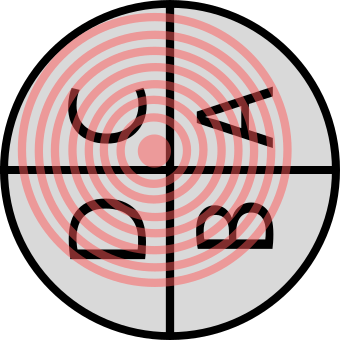
\includegraphics[height=0.5\linewidth, angle=270]{QPD_diagram.png}
	\caption{Diagram depicting a typical QPD interface. The four 
		quadrants of a QPD experience different photocurrents based 
		on the total intensity of light incident on each section 
		(labelled A, B, C, D).}
	\label{fig:QPD_diagram}
\end{figure}

Now while the signal returned by the QPD is proportional to the particle's
displacement it cannot be directly interpreted as such until converted
from voltage units to displacement units. This can be done by taking the 
ratio of the expected diffusion coefficient $D_{exp}$ and the diffusion 
coefficient calculated by calibration $D_{cal}$.
\begin{align}
	\label{eq:conversion_factor}
	D_{exp} = \frac{k_BT}{6\pi\eta a} \Rightarrow Conversion\ Factor \ [m/V]= \sqrt{\frac{D_{ext}}{D_{cal}}}
\end{align}

The former depends on the exact size and shape of the target particle, 
using image analysis one can get a fairly accurate estimation of the particles radius (a). The latter can be determined from fitting the QPD signal to a given model, for computing the diffusion coefficient 
computing the auto correlation function, the mean square displacement, 
or taking the power spectrum are used. The former two are ideal for 
simple position detection systems, where the QPD reports the signal at 
each time step, however they often require longer recording times in 
order to reach an ideal accuracy. More sophisticated QPD systems can calculate the power spectra of an incoming signal and immediately fit 
it to a power spectrum. Once the conversion factor is known any further 
QPD signals can be converted immediately into displacement units to monitor
the position of the target particle, the spacial resolution being  
limited by the accuracy of the calibration method. A full tutorial in 
maximising the accuracy of the power spectral method is provided by 
Berg and Sorensen \cite{BergSoerensen2004}

For our consideration we will be relying on the power spectrum method 
to characterise the motion of the trapped particle. Firstly because
it is sometimes integrated into QPD systems. And secondly, because 
on of the main advantages of the power spectrum method is its shorter 
calibration times, and the ability to filter out large sources of signal 
noise. 

%%%%%%%%%%%%%%%%%%%%%%%%%%%%%%%%%%%%%%%%%%%%%%%%%%%%%%%%%%%%%%%%%%%%%%%%%%%%
%%%%%%%%%%%%%%%%%%%%%%%%%%%%%%%%%%%%%%%%%%%%%%%%%%%%%%%%%%%%%%%%%%%%%%%%%%%%
\section{Modelling the QPD response signal of a non-spherical particle}
In order to simulate a typical experimental set up with a QPD 
installed as a position detection system we need to evaluate 
the total magnitude of the electric field incident on the 
photo-diode surface. While trapping a micro-particle, the 
scattered and incident fields combine together and interfere 
with one another. These fields are collected by a condenser 
lens in the far field limit and are focused onto the QPD 
surface, the total intensity can be evaluated as:
\begin{align}
	I(x,y) = \epsilon_0c\left|
	\begin{bmatrix} 
		E_{i,x}(x,y)+E_{s,x}(x,y) \\ 
		E_{i,y}(x,y)+E_{s,y}(x,y) \\ 
		E_{i,z}(x,y)+E_{s,z}(x,y)
	\end{bmatrix} \right|^2 \times step(\theta_{NA}-\theta(x,y))
\end{align}

The last term is simply a representative step term that defines 
the outer limit by which we evaluate the electric field, this is 
analogous to a condenser lens removing noise from other light 
sources by only accepting light at a specific acceptance angle 
defined by its numerical aperture $NA_c$. Depending on the 
relative size of our particle we can adjust the acceptance angle, 
this has very little effect on the transverse signals, but for 
axial evaluations of a trapped particle the numerical aperture 
should be tuned so that the resultant response curve has negative 
slope in order to allow for axial position detection, the method 
for finding this angle $\theta_\Theta$ is discussed in 
\cite{Friedrich2012}.

The incident beam is simple enough to define given our set up 
parameters, for the sake of simplicity we assume that our beam is a 
Gaussian beam. \textit{Ott} uses a point matching approach to 
approximate the beam shape coefficients of the incident field by 
fitting it to the far field estimate. From the QPD's perspective 
it is receiving light both from the incident and scattered beam simultaneously, as such both fields must be expressed using outgoing 
vector spherical harmonics.
\begin{align}
	E_{\rm inc}(r)&=
	E_0\sum^\infty_{n}\sum^n_{m=-n}\left[a_{mn}{\bf M}^{(2)}_{nm}({\bf r})+
	b_{nm}{\bf N}^{(2)}_{nm}({\bf r}) \right] 
	\\
	E_{\rm scat}(r)&=E_0 \sum^\infty_n \sum^n_{m=-n} \left[
	p_{nm}{\bf N}_{nm}^{(2)}({\bf r})+q_{nm}{\bf M}_{nm}^{(2)}({\bf r})
	\right] 
\end{align}

Where the superscript (2) denotes an outgoing spherical harmonic
function. In order to compute the scattering from the target particle \textit{ott} uses the $T$-matrix method, this is not essential 
for a simple sphere but is essential for complex shaped particles 
such as dimers. The scattered and incident fields are then combined 
together in the far field to get $I(x,y)$, the quadrant and overall 
signals are calculated via:
\begin{align}
	Q_i &= \sum_{n,m} I(x_{i,n}, y_{i,m}) \\
	S_{x} &= \frac{(Q_1+Q_2)-(Q_3+Q_4)}{\sum I_0(x,y)} \\
	S_{y} &= \frac{(Q_1+Q_3)-(Q_2+Q_4)}{\sum I_0(x,y)} \\
	S_{z} &= \frac{(Q_1+Q_2+Q_3+Q_4}{\sum I_0(x,y)}
\end{align}

Where the denominator is the total intensity on the QPD while there is 
no particle within the trap. You would expect that $S_x$ and $S_y$ are
near identical for equal particle displacements, however due to the 
polarisation of the beam there will be a slight bias to the signals 
for motion along the direction of the polarisation vector. This is 
generally not an issue if the particle trajectory is sampled for a 
long enough time period. By converting from signal units to length
units (see Eq.\eqref{eq:conversion_factor}) the trap shape can be 
discerned from the QPD signals, assuming the fluid properties are
known to a high degree of accuracy.

While translational motion has no knock on effects to the QPD signal, 
rotational changes are double counted by both the incident and total 
field. This results in rotational motion being biased in the QPD signal 
- even when collecting signals from isotropic scatterers. To prevent 
this we rotate the total field via the inverse rotation matrix of the 
dimer.

To confirm that our method is producing accurate results, we ran a
comparison test between our simulative QPD and the results from \cite{Rohrbach2002}. Where a $300\ nm$ diameter sphere is scanned 
across the path of a focused Gaussian beam ($\lambda=1064\ nm$, $NA=1.2$), the sphere has a refractive index of 1.57 and is suspended in water ($n_{med}=1.33$) and the condenser lens has its numerical aperture
set to 0.5 ($\theta_{max} = 30^\circ$). Scanning across all three primary axis produced the following response curve:
\begin{figure}[h!]
	\begin{subfigure}{0.475 \linewidth}
		\subcaption{}
		\includegraphics[width=\linewidth]{QPD_axial_tests.png}
	\end{subfigure}
	\begin{subfigure}{0.475 \linewidth}
		\subcaption{}
		\includegraphics[width=\linewidth]{QPD_lat_tests.png}
	\end{subfigure}
	\caption{Comparison between QPD response signal versus work conducted by 
		Rohrbach, single sphere ($r = 150\ nm$, $n=1.57$) is scanned by a $1064\ nm$ laser and the QPD signal recorded. Solid lines represent the signal produced by QPD using \textit{ott} and points represent the signal response collected from \cite{Rohrbach2002}.}
	\label{fig:Rohrbach}
\end{figure}

The discrepancy between our simulated QPD and the results 
from Rohrbach can be attributed to the fact that the position 
to signal error grows as you move further from trap focus. 
As the particle moves further from the trap focus the error 
in the attributed signal grows substantially \cite{Rohrbach2002}.
In most optical trapping experiments we usually are calibrating 
a strong trap where the mean square displacement falls well within 
the linear regime shown in fig.~\ref{fig:Rohrbach}. In which case 
the error between Rohrbach's model and our own is inconsequential 
for calibration purposes. 

%%%%%%%%%%%%%%%%%%%%%%%%%%%%%%%%%%%%%%%%%%%%%%%%%%%%%%%%%%%%%%%%%%%%%%%%%%%%
%%%%%%%%%%%%%%%%%%%%%%%%%%%%%%%%%%%%%%%%%%%%%%%%%%%%%%%%%%%%%%%%%%%%%%%%%%%%
\section{Characterisation of asymmetric dimer dynamics via PSD analysis}
\label{sec:PSD_analysis}
While it is possible to extract all of the relevant dynamics from a simulation, from an experimental standpoint characterising those 
dynamics is dependent on what experimental techniques are used. 
Translational motion can be characterised via a position detection 
system but angular motion is far more difficult to detect, let along characterise. 

The tweezer setup we are simulating incorporates a dual objective 
configuration, using one objective lens to focus the beam (NA=1.25)
where as the condenser lens acts as a means of truncating the electric
field ($NA_c=0.25$). The electric field falling onto the QPD surface is computed by considering the far field of the combined incident and 
scattered beams. We can ignore any contributions from the electric
field that falls outwith the maximum acceptance angle of our condenser
lens ($\theta_{max}\approx\pm10.8\deg$). This is not perfectly analogous
of a true QPD as external factors (i.e. internal resistance, external
light sources, and vibrations) would also contribute to the detected QPD 
signal. It does provide us a means of showing what elements of a particle's
trajectory are represented in the power spectrum and which elements are 
obscured.

As a benchmark we start by considering a single sphere within an optical 
trap. A single polystyrene sphere suspended in water ($a=1\mu m$, 
$n_p=1.59$, $n_m=1.33$) was trapped by a focused Gaussian beam ($NA=1.25$) using circularly polarised light. For the sake of time efficiency the trajectory was sampled every 10 time steps, meaning the upper bound on 
the power spectra is $f_{Nyq}=f_{sample}/2=5000\ Hz$. To optimise the 
frequency window we fitted the power spectra using the aliased Lorentzian.
(Eq.~\eqref{eq:aliased_lorentzian}). 
\begin{figure}[h!]
	\centering
	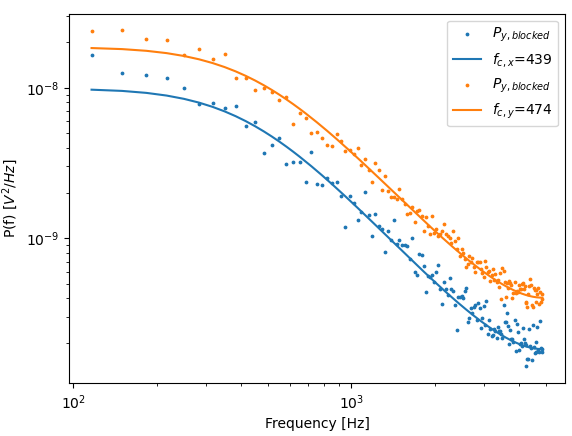
\includegraphics[width=\linewidth]{PSD_sphere.png}
	\caption{Recorded power spectra fitted to eq.~
		\ref{eq:alaised_lorentzian}, scattered points represents 
		the blocked data ($n_b=100$). Corner frequency for the 
		Lorentzian curves are reported in the legend.}
	\label{fig:psd_sphere}
\end{figure} 

As shown in fig.~\ref{fig:psd_sphere}, the two power spectra 
report different corner frequencies which would be indicate 
that the trap is not perfectly circular. We can use both 
\textit{ott} and the trajectory itself to derive an estimation 
of the trap geometry. Additionally, we fitted the 
same Lorentzian to the sphere's positional data, this would be a
situation when the QPD signals are completely uncorrelated with 
one another and there is a constant ratio between the QPD signal 
and the sphere's position. The corner frequencies and corresponding 
trap stiffness are reported below:

\begin{center}
	\captionof{table}{QPD fitting for single sphere}
	\label{tab:sphere}
	\begin{tabular}{ |c|c|c|c|c|c|c| } 
		\hline
		Fitting parameter & \multicolumn{2}{|c|}{\textit{ott} estimates} 
		& \multicolumn{2}{|c|}{QPD fitting} & \multicolumn{2}{|c|}{Trajectory 
			fitting}\\
		\hline
		$f_c\ [Hz]$ & 447 & 450 & \parbox{1cm}{\centering 439} & 474 
		& \parbox{1.25cm}{\centering 523} & 513 \\
		$\sigma(f_c)\ [Hz]$ & --- & --- & 9.30 & 9.65 & 8.67 & 8.61 \\
		$\kappa\ [pN/\mu m]$ & 53.05 & 53.40 & 51.96 & 56.09 & 61.94 & 60.7 \\
		\hline
		Ellipticity &
		\multicolumn{2}{|c|}{8.16 \%} &
		\multicolumn{2}{|c|}{27.17 \%} &
		\multicolumn{2}{|c|}{13.8 \%} \\
		\hline
		
	\end{tabular}
\end{center}

Where $\sigma(f_c)$ is computed from \cite{BergSoerensen2004}, 
where the variance is based upon our choice of frequency 
boundaries ({$f_{min}:f_{max}$} = {$100\ Hz: 5000\ Hz$}). And 
the ellipticity of the beam is given by $e = (1-\kappa_y/
\kappa_x)^{0.5}$ and is a measure of the symmetry of the beam 
wavefront. Its clear from these initial results that the QPD 
is more sensitive to changes along the y-axis than the x-axis 
when compared to the direct \textit{ott} calculations. This is 
somewhat reflected in the trajectory results. Typically, even 
an industrial Gaussian beam will produce an elliptical diffraction 
limit spot when heavily focused; in their tutorial for optimizing 
the PSD analysis, Berg and Sorensen reported a ellipticity of 
around 15 \% after a total calibration time of 80 seconds 
\cite{BergSoerensen2004}.

The reason for the discrepancies between all 3 methods is due 
to what is actually being measured. The \textit{ott} estimates 
are simply looking at the change in the trapping force as you
move along a given axis'. In reality, a particle will be freely
diffusing within the trap focus meaning over a short calibration 
time the QPD is only estimating a weighted average of the trapping
strength. If calibrated over an long enough time frame you would 
expect that the resulting power spectra would exactly mirror the 
\textit{ott} predictions. There is a clear trade off in terms of 
accuracy and computation time as shorter calibration runs are 
computationally more efficient but prone to errors. However, it
should be noted that the estimation made by the QPD is still less
than the results from \cite{BergSoerensen2004}, though this could
be due to a lack of external noise signals.

With this in mind, let us consider a symmetric dimer that is 
optically trapped by the same Gaussian beam. Not only does 
the dimer's equilibrium position change but it is subjected 
to rotational motion due to its unequal moments of inertia. 
This is reflected in the calibration results using the simulated 
QPD, where we see a drastically different estimation between the 
\textit{ott} estimate and the QPD estimate.
\begin{center}
	\captionof{table}{QPD fitting for symmetric dimer}
	\label{tab:dimer}
	\begin{tabular}{ |c|c|c|c|c|c|c| } 
		\hline
		Fitting parameter & \multicolumn{2}{|c|}{\textit{ott} estimate} & 
		\multicolumn{2}{|c|}{QPD fitting} & \multicolumn{2}{|c|}{Trajectory fitting} \\
		\hline
		$f_c\ [Hz]$ & 445 & 409 & \parbox{1cm}{\centering 431} & 424 
		& \parbox{1.25cm}{\centering 274} & 285 \\
		$\sigma(f_c)\ [Hz]$ & --- & --- & 9.22 & 9.16 & 7.82 & 7.91  \\
		$\kappa\ [pN/\mu m]$ & 52.82 & 48.54 & 51.13 & 50.26 & 32.45 & 33.75 \\
		\hline
		Ellipticity &
		\multicolumn{2}{|c|}{28.5 \%} &
		\multicolumn{2}{|c|}{12.7 \%} & 
		\multicolumn{2}{|c|}{13.8 \%} \\
		\hline
	\end{tabular}
\end{center}

Now we see that the \textit{ott} predicts a more elliptical 
trap compared to the QPD model which says the trap is far
more symmetrical while trapping a symmetric dimer. A potential 
reason that \textit{ott} no longer expects a circular trap 
is because that unlike a sphere, the force displacement 
curve is not strictly harmonic. If we consider a dimer that 
is some distance from the beam axis, the sphere closest to 
the trap focus will experience a slightly greater force 
compared to the sphere further from the trap. As such its not
accurate to assume that the external force $F(x) = \kappa x$
instead we must consider that it is a function of both the 
position and orientation simultaneously. 

There is still a concern in the fact that both produce similar
power spectra, enough so that it would be difficult to determine
if a trapped particle was actually a dimer or a sphere. This is
because the rotational and translational motion, coupling of the 
has been highlighted previously \cite{Vigilante2020}, but there 
effects have not been demonstrated in the context of an experimental situation. We can see from the difference in trajectory and QPD 
fittings that while our description of the trap shape is very 
similar (both methods give similar ellipticity values) but the 
magnitude of the trap strength are significantly different. This 
is partially explained by the fact that the QPD is not actually 
measuring the position of the particle but instead the intensity 
distribution of the total field incident on the QPD surface. In 
which case if the dimer is rotated slightly the QPD signal will 
change even if the dimers centre of diffusion remains stationary. 
%%%%%%%%%%%%%%%%%%%%%%%%%%%%%%%%%%%%%%%%%%%%%%%%%%%%%%%%%%%%%%%%%%%%%%%%%%
%%%%%%%%%%%%%%%%%%%%%%%%%%%%%%%%%%%%%%%%%%%%%%%%%%%%%%%%%%%%%%%%%%%%%%%%%%

\section{QPD for angular displacement detection}
\label{sec:angular_displacement}
The next logical step is to consider whether or not a QPD can at 
all be utilised for detection of rotational motion. This has been
shown for nano-particles that exhibit periodic rotational motion
using by considering the difference in diagonal quadrants 
\cite{Yifat2021}. The only difference between these results is 
the fact that rotation occurs perpendicular to the particle's long 
axis, whereas dimers rotate about their long axis. The benefit of 
detecting rotational motion is that one can begin to build a better understanding about how angular momentum is transferred to a dimer 
which could be extended to more complex particles. This could give 
some understanding to the results of Chapter 4. 

At just a cursory glance it would appear that there is a clear
relationship between the QPD signal and the orientation of the 
dimer. If we look at the QPD signal produced by a dimer as it is 
rotated we can see that it is equally sensitive to rotations in
either the X-Z or Y-Z plane but there is no change in the signal 
when rotated by in the X-Y plane. 
\begin{figure}
	\centering
	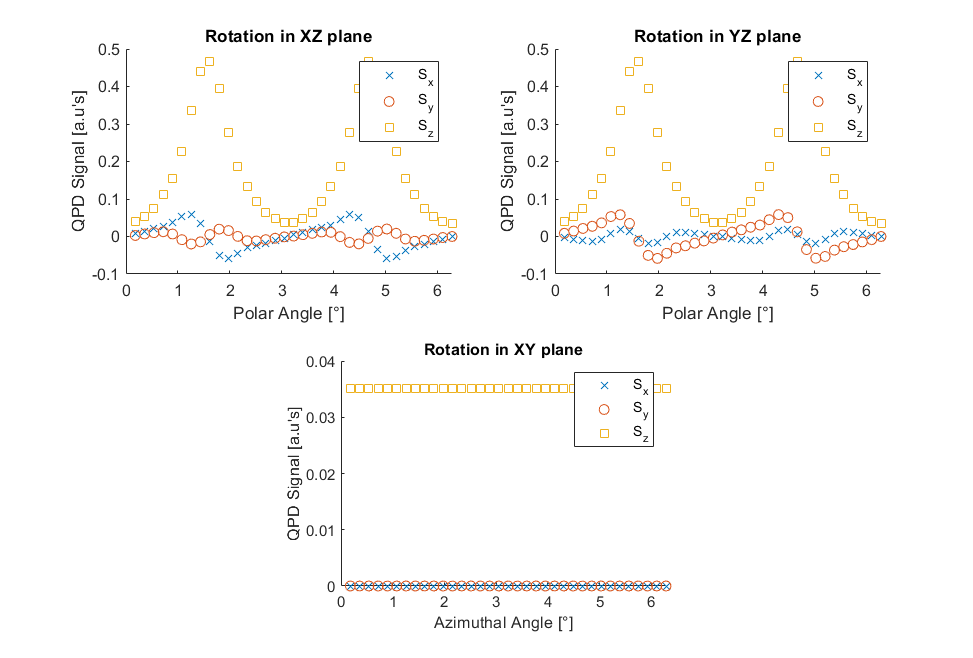
\includegraphics[width=0.9\linewidth]{rotation_figure.png}
	\caption{QPD signals detected by a dimer being rotated while
		centred at the focus of the optical trap. Top right:
		rotation in the X-Z plane. Top left: rotation in the
		Y-Z plane. Bottom: Rotation in the X-Y plane.}
	\label{fig:QPD_rotation}
\end{figure}

However if we compare this to fig.~\ref{fig:Rohrbach} we can see 
that the the signal change is dwarfed by the translational motion. 
So while their is a clear relationship between the two trying to
discern between translational and rotational contributions to the
QPD signal is not a simple task. This is significant because it 
means that with regards to the power spectrum fittings in Table 
\ref{tab:dimer} there is no means of discerning between that of 
a trapped sphere and that of a trapped dimer. Furthermore the 
dynamics reported by the power spectrum fitting do not accurately 
reflect the actual dynamics of the dimer, instead only providing 
a orientation-averaged trap strength. But unless we have some means
of at least estimating the degree of rotational freedom, calculating
the actual trapping strength is impossible. 

The dependence of $S_x$ and $S_y$ and the dimer's orientation
(defined by the spherical angles $\theta$, $\phi$) is therefore
not clear. To that end, we utilised machine vector regression,
which takes as an input the voltage from the 4 quadrants and 
tries to fit that to the dimer's trajectory. We utilised the 
scikit-learn module available in Python to transform the 4D vector
of the QPD signal to a 2D vector specifying the expected displacement
of the target particle. Unlike in Chapter 4 where we utilised 
machine learning to get a probabilistic estimation of the 
particle's orientation we utilise vector regression as we 
want to replicate QPD precision as closely as possible. 

In order to fit the QPD signal to dimer displacements we need
to train our model. For each size ratio considered a 3 second
trajectory was ran (using the same conditions in 
Sec.~\ref{sec:PSD_analysis}) and a normal distribution of the 
dimer's position was taken and used to construct a training 
data set of QPD signals. After the training results reached an
error rate of less than 1\% the same trajectory was used to
construct a test set that would allow our model to fit the QPD 
signal to the positional data from the trajectory. Fitting the 
QPD signal to the dimer's position showed promising results, 
shown in fig~\ref{fig:QPD_rotation} is a prediction of a 
symmetric dimer's position based on the QPD signal. With the 
actual displacement on the x-axis and the predicted result y-axis, 
and the dashed line represents the y=x line - indicating an 
ideal prediction. 
\begin{figure}[h!]
	\centering
	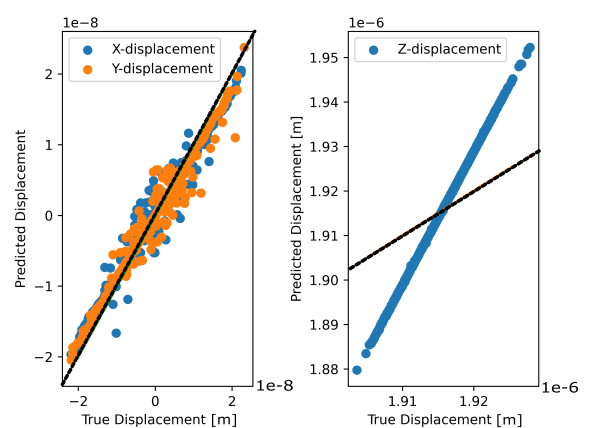
\includegraphics[width=0.9\linewidth]{predicted_displacements.png}
	\caption{Scikit-Learn's best predictions of the displacement 
		of a symmetric dimer placed in an optical trap, predictions 
		are based on the QPD signal collected at the 4 quadrants. 
		(Left) predictions of the $X$ \& $Y$ displacements. 
		(Right) predictions of the $Z$ displacement, predictions 
		have been scaled so they represent the displacement from 
		the beam focus. The dashed black line represents when the 
		predicted displacement = the true displacement.}
	\label{fig:predicted_displacements}
\end{figure}

Fig~\ref{fig:predicted_displacements} shows that its relatively 
trivial to predict a particle's position based off the QPD signal
in the $X$-$Y$ plane but harder along the axial direction. If we 
consider Fig~\ref{fig:Rohrbach} we note that the change in signal
strength is only truly linear close to the beam focus, as shown in
Chapter 3, dimers do not trap close to the beam focus but further 
away. This would suggest that the model cannot accurately predict 
the displacement of a dimer in the axial direction as there is a 
non-linear relationship between the change in signal and the change 
in axial position. It should be noted that even in the worst case 
the difference between the predicted and true displacements is 
around $~20 nm$. 

These displacements are relative to the trap focus and 
so accurate tracking of the beam movements needs to be taken if 
you want to consider the displacement relative to some larger object. 
These results are likely due to the fact that displacement and 
signal units are linearly related by \eqref{eq:conversion_factor}. Interestingly when we run the same protocol for different sized 
dimer's there seems to be a cut off point when the fit begins to 
fail. We can compute the coefficient of determination ($R^2$) for 
our model's prediction, the $R^2$ for each fit vs its size ratio 
shows that beyond a size ratio of 5 the machine learning begins 
to fall off significantly.
\begin{figure}[h!]
	\centering
	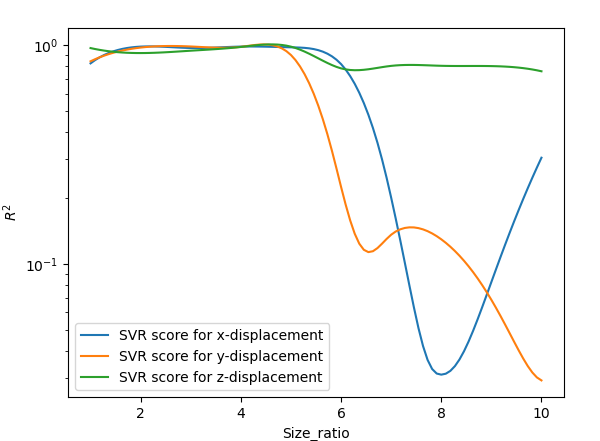
\includegraphics[width=\linewidth]{score_results.png}
	\caption{The coefficient of determination for different sized 
	dimers using the scikit-learn vector regression model. Each line
	plot shows the $R^2$ value for either the $X$, $Y$, or $Z$ 
	displacements. When the size ratio is greater than 5 the $R^2$ 
	value falls off dramatically, from around 0.95 down to as low as 
	0.01.}
\end{figure}

This is surprising because we would expect that as the second 
sphere shrinks the dynamics should more closely approximate that 
of a single sphere. This should be reflected in the total field
incident on the QPD and therefore the machine learning program 
should be able to easily detect the dimer's translational motion.
We can therefore only conclude that the contribution that the 
second sphere makes to the scattered beam is not proportional to
its size. What is interesting is that the axial prediction does 
not experience as a large a drop in accuracy, suggesting that the
total field incident on the QPD is not changing drastically, but
rather that the second sphere is altering the distribution such
that the $X-Y$ displacements are being incorrectly predicted. 
This could simply be a limitation of the \textit{mstm} software being 
unable to accurately represent the T-matrix of the second sphere, 
however the documentation does not specify any limits on the relative 
size differences so it is unclear if this is a known issue. The 
problem is that it is difficult to verify the error between the 
\textit{mstm} predicted scattering and the true scattering without 
replicating the exact system experimentally. For now we can say that predictions for size ratios greater than 5 should be for the most 
part disregarded. 

Detection of rotational motion was attempted using the same method, 
the model was trained on the same trajectory mentioned in 
\ref{sec:off-axis}, where the dimer is trapped in an off-axis 
orientation. We chose this trajectory instead of a strictly vertical
orientation in order to confirm that the model can distinguish between 
the polar angle and the azimuthal angle. The results of which are 
are shown in Fig.\ref{fig:predicted_rotations}
\begin{figure}[h!]
	\centering
	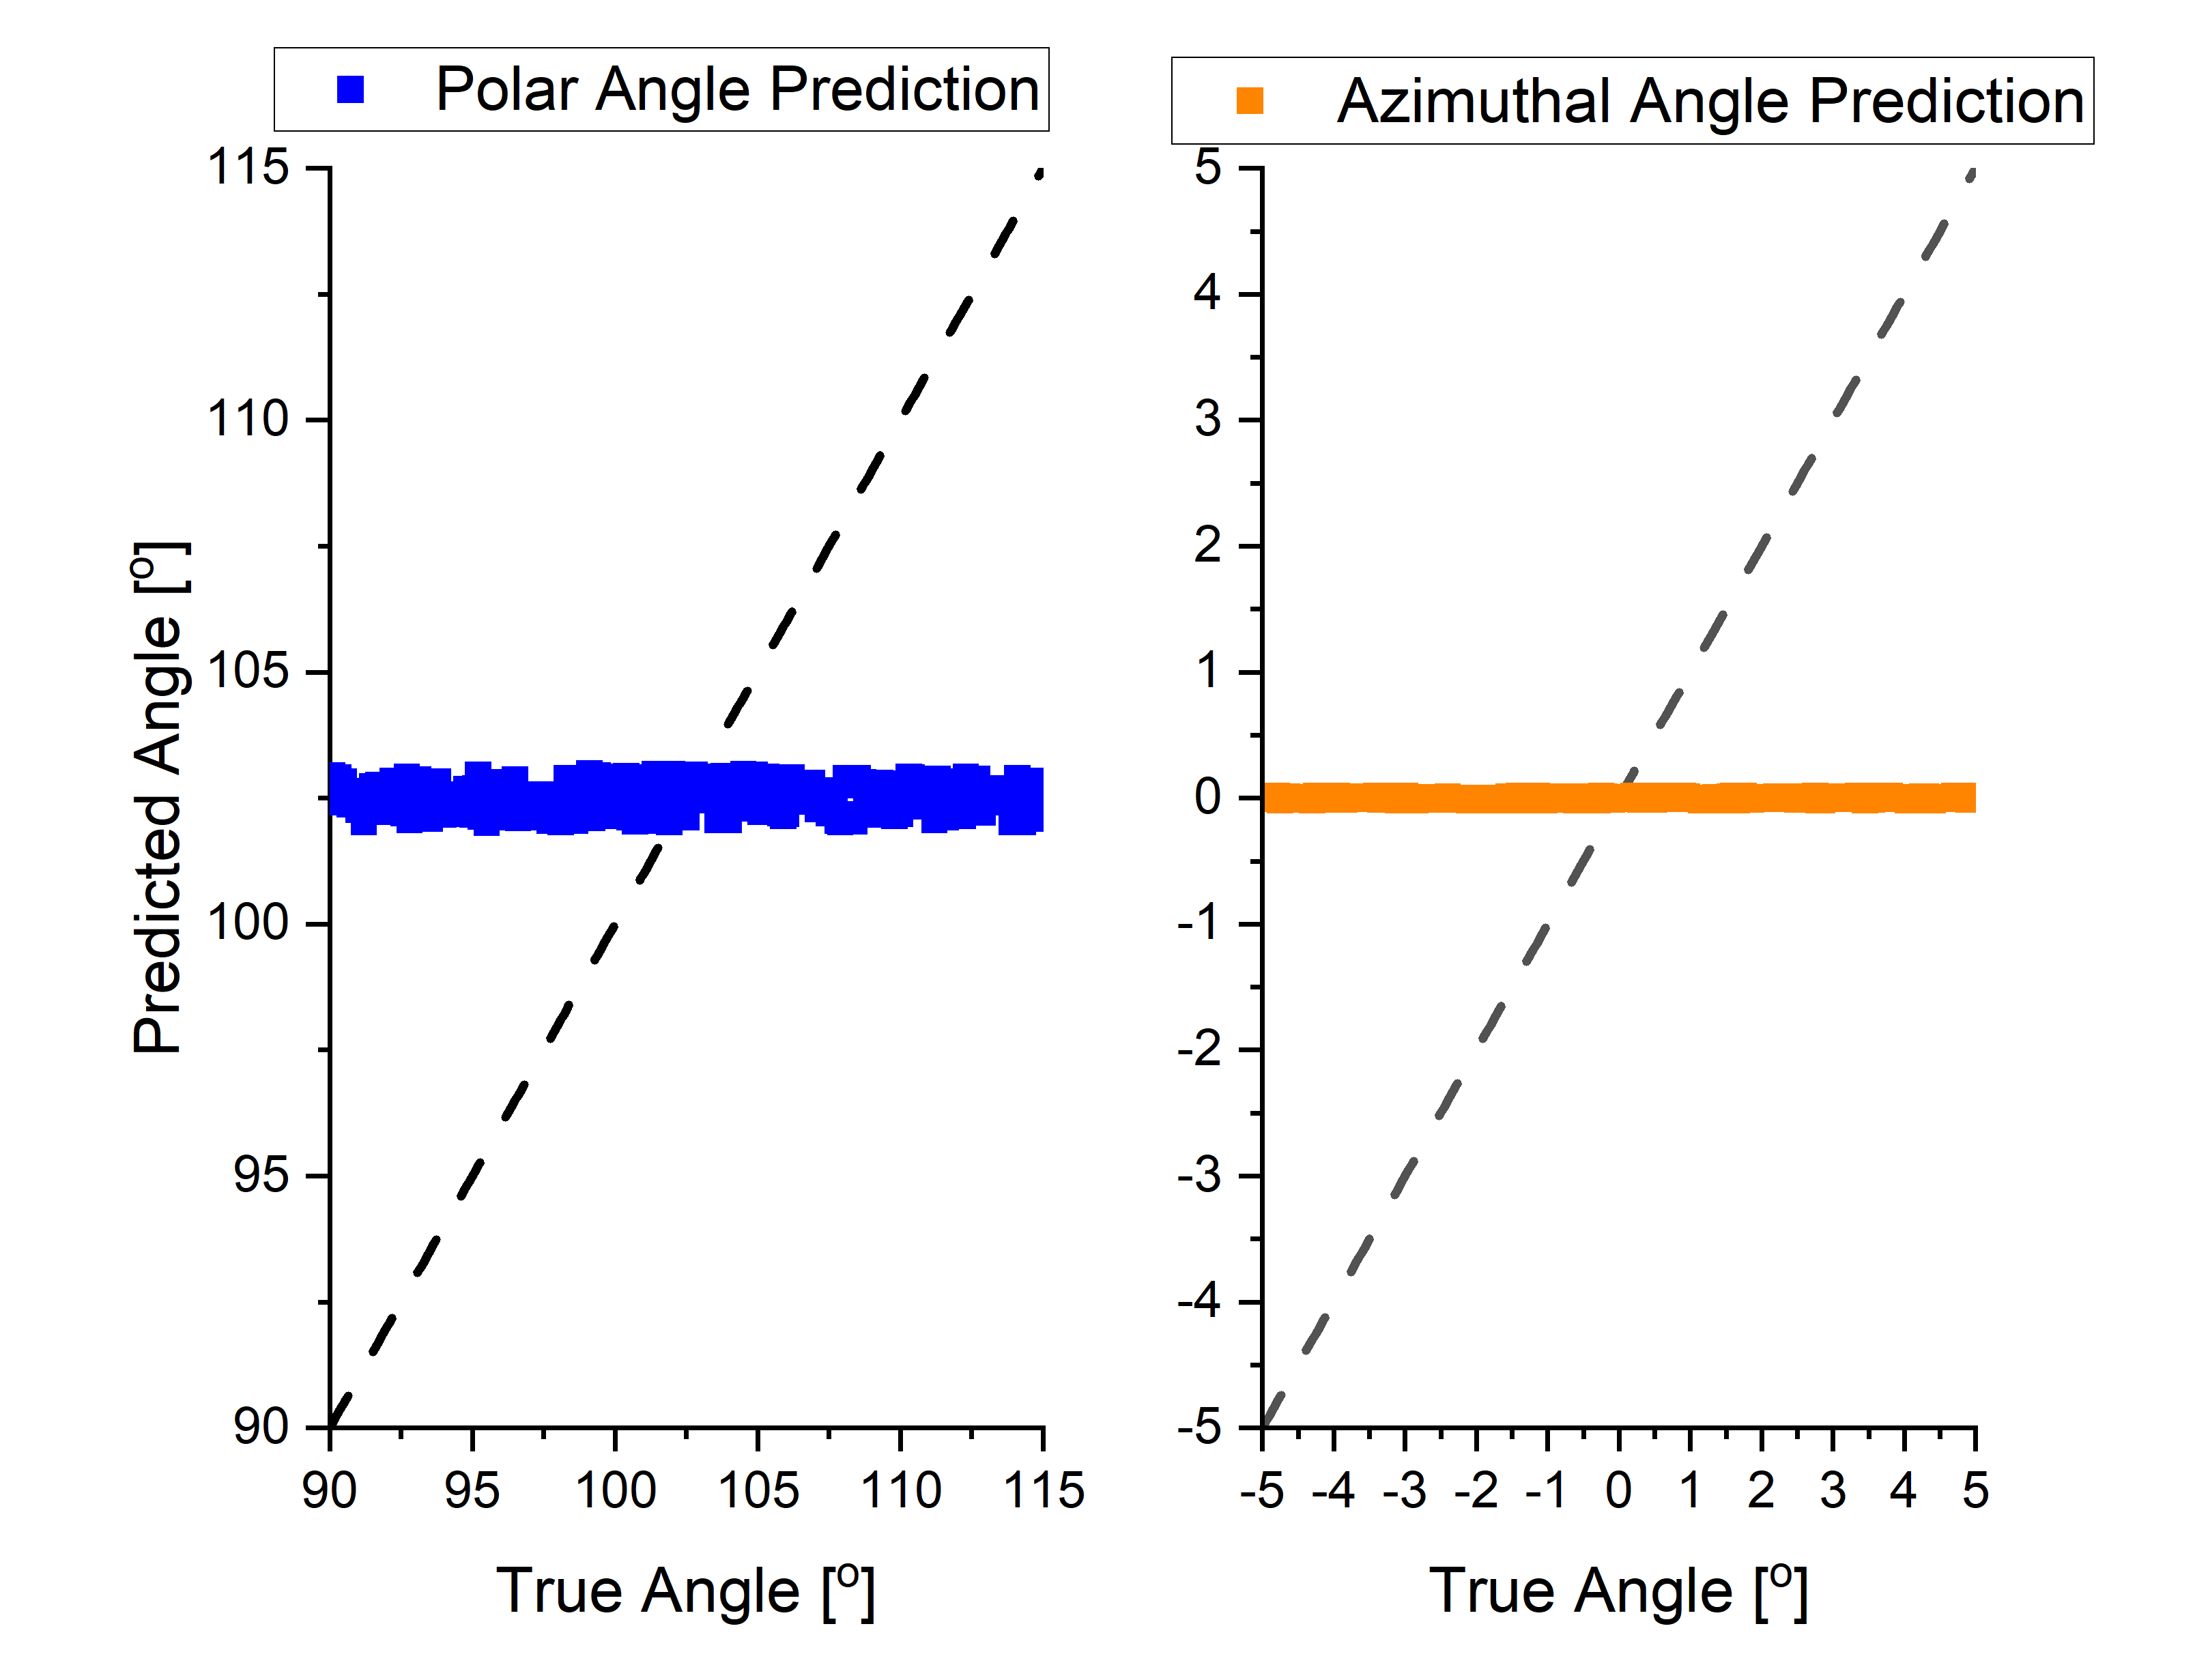
\includegraphics[width=\linewidth]{angular_predictions.png}
	\caption{Scikit-learn's prediction of the sphericical angles of
	a dimer trapped in an off-axis configuration (see Sec\ref{sec:off-axis}).
	(Left) predictions of the azimuthal angle, (Right) predictions 
	of the Polar angle. Dashed black lines show the ideal prerformance 
	where the predicted angle = true angle.}
	\label{fig:predicted_rotations}
\end{figure}

From here we can see that the vector regression model performs rather
poorly in predicting the rotations made by the dimer, even in a situation
where visibly the dimer is an off-axis orientation. While the model can 
roughly predict the median polar angle (~$102\deg$) it has no means of
predicting the rotations made by the dimer. This result is reveals two important factors: Firstly, the change in the QPD signal for rotational
motion is a full order of magnitude smaller than the change in signal 
for translational motion meaning the model has no means of distinguishing
between large and small rotations. Secondly, is the fact that unlike 
translational motion, rotational motion is dependent on the prior 
orientations in the trajectory. This was already discussed in Chapter 4
where we improved our machine learning model by accounting for the 
the priors $p(\hat{\bf n}_\alpha)$, where we weighted our estimation 
by the distance from our prior estimate. Vector regression is powerful
for predicting uncorrelated events but has no means for accounting for
cases where one event is dependent on the next. At the same time, 
utilising machine learning in the case of a QPD would not be able to 
provide a high enough orientational resolution without first sampling 
from a trajectory and creating a unique set of reference orientations
(see Sec.~ \ref{sec:ref_orientations_explained} for definitions).

Overall, the reliance on machine learning to perform vector 
regression on the collected scattered field is not a viable 
method for detecting let along characterising the angular 
displacement of an isotropic scatterer. While there is a 
clear correlation in the scattered signal and angular 
displacement the translational motion makes up the majority 
of the expected signal detected by the QPD. As of now, there
is no optical arrangement that would allow rotational motion 
while restricting translational motion. 

\section{Conclusion}
We have developed a program that allows one to compute the QPD 
response signal produced by an arbitrary shaped particle. By 
utilising \textit{mstm} we can construct any combination of 
spherical particles and measure the total field incident on the
focal plane of the condenser lens. This has immediate applications 
in replicating power spectral data from complex particle structures 
that experience periodic rotational motion. Furthermore, if all 
contributions to the QPD response signal are known it would allow 
researchers to compare the reported dynamics given by an experimental
QPD to that of our simulated response signal. 

The QPD module shows promising results for dimers who have a size 
ratio less than 5. Utilising vector regression models allowed for 
accurate predictions of the displacements made by dimers while 
confined by an optical trap. The use of vector regression is necessary
to return a continuos range of positions instead of a probabilistic
approximation of the particle's position vector. 

As shown in \ref{sec:angular_displacement} random rotational motion 
is difficult to distinguish from random translational motion. Even
when utilising a vector regression model the angular displacement
predicted does not match the trajectory data. This means that at least
for now utilising focal plane interferometry cannot provide an 
accurate estimation of angular displacements. While static light 
scattering methods - as seen in Chapter 4 - do present a possible 
alternative, the limited angular resolution due to a high mixing 
of signal and orientation spaces also make the method difficult to 
implement. Measurements of angular displacement are crucial for 
measuring torques exerted on trapped particles, current torque 
measurements assume that only the the polarisation contributes to 
the applied torque, measuring non-polarisation related torques still 
eludes us. 

Overall, tracking the angular displacements of non-spherical 
objects for the purposes of torque measurements will require 
further study. Fully understanding the torques applied to an 
arbitrary shaped particle would pave the way for high-precision 
particle-manipulation techniques and a greater understanding 
of the interactions between focused beams and aggregate particles.

 
